% Heine らの体積データの説明と、時間の対応の決め方、今後の使い方（日本語、自分用）
%
% ビルド: lualatex slides_volume_ja.tex （2回）
% 図: python ansys_usermat/apdl/volume_figs.py（data/heine_volume/ の集計から）
% データは集計だけ（条件 × 日の平均と SD）。反復ごと・画像ごとの値は載せない（請求に応じて提供）。
\documentclass[aspectratio=169,11pt]{beamer}
\usepackage{luatexja}
\usetheme{Madrid}
\usecolortheme{seahorse}
\usepackage{amsmath,amssymb}
\usepackage{booktabs}
\usepackage{xcolor}
\graphicspath{{assets/}}
\definecolor{c3}{RGB}{30,80,160}
\setbeamercolor{frametitle}{bg=c3, fg=white}
\newcommand{\pt}[1]{\colorbox{c3!10}{\parbox{0.96\linewidth}{\small #1}}}

\title{Heine らの体積データ}
\subtitle{中身、時間の対応の決め方、今後の使い方（自分用）}
\author[西岡佳祐]{西岡佳祐}
\date{2026年10月14日}

\begin{document}
\maketitle

% --------------------------------------------------------
\begin{frame}{このデータは何か}
\small
\begin{itemize}\setlength{\itemsep}{3pt}
  \item \textbf{測り方}：LIVE/DEAD 染色（SYTO9 と PI）したバイオフィルムを共焦点顕微鏡（CLSM）で撮影し、
        画像から \textbf{バイオフィルムの体積}と\textbf{生きた割合}を出したもの。Heine さん（MHH）から 10 月 13 日に届いた。
  \item \textbf{体積の単位}：$10^6\,\mu$m$^3$。\textbf{画像 1 枚の視野の中}のバイオフィルムの体積（1 個のコロニーではない）。
  \item \textbf{数}：画像 5 枚 = バイオフィルム 1 個。1 時点あたり 3〜9 個。毎回、別のバイオフィルムを壊して測る。
  \item \textbf{条件}：4 条件（CS、CH、DS、DH）× 6 時点（Day 1、3、6、10、15、21）。
  \item \textbf{使う量}：FEM は代表的なバイオフィルム 1 個を解くので、\textbf{日ごとの平均とバイオフィルム間の SD}。
        画像ごとのばらつきは使わない。
  \item \textbf{公開の決まり}：生データは請求に応じて提供（Heine さんの希望）。リポジトリには集計だけ（論文の図と同程度）。
\end{itemize}
\pt{推定（第 3 章、EML）は組成と生きた割合だけを使い、体積は使っていない。体積は\textbf{成長の変数 $\alpha$} の側に対応する。}
\end{frame}

% --------------------------------------------------------
\begin{frame}{体積：条件ごとの変化}
\centering
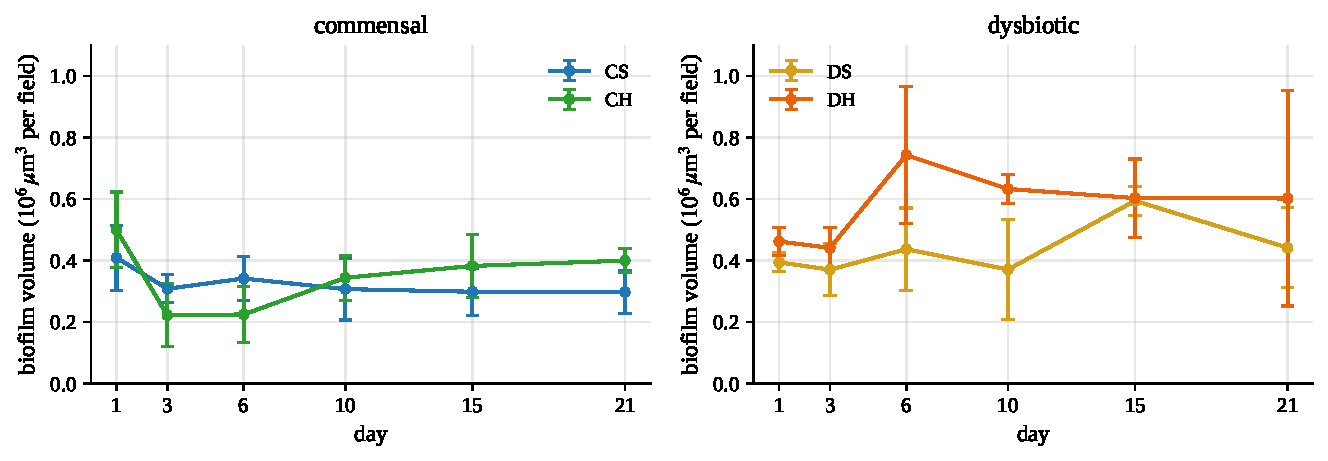
\includegraphics[width=0.9\linewidth]{fig_vol_volume.pdf}\\[2pt]
\begin{itemize}\small
  \item 常在（左）：CS は減り続ける。CH は Day 3 で一度減り、その後ゆっくり増える。
  \item dysbiotic（右）：DS は増えたり減ったり。DH は Day 6 まで急に増え、その後は横ばいか少し減る。
  \item エラーバーはバイオフィルム間の SD。ばらつきは大きい（とくに DH の Day 21）。
\end{itemize}
\end{frame}

% --------------------------------------------------------
\begin{frame}{生きた割合と、種ごとの生きた体積}
\begin{columns}[c]
\begin{column}{0.4\textwidth}
\centering
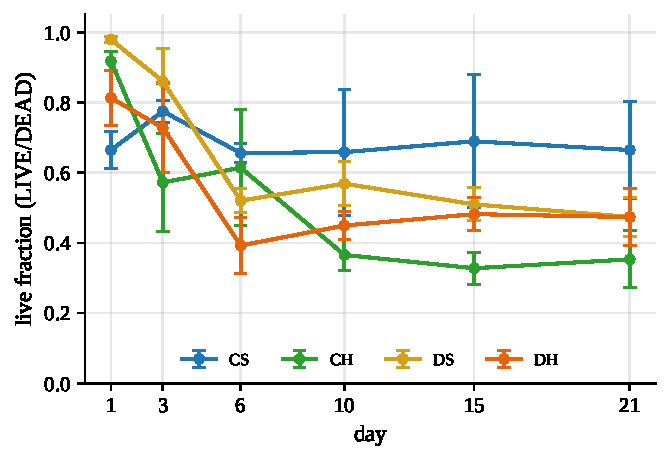
\includegraphics[width=\linewidth]{fig_vol_live.pdf}
\end{column}
\begin{column}{0.58\textwidth}
\centering
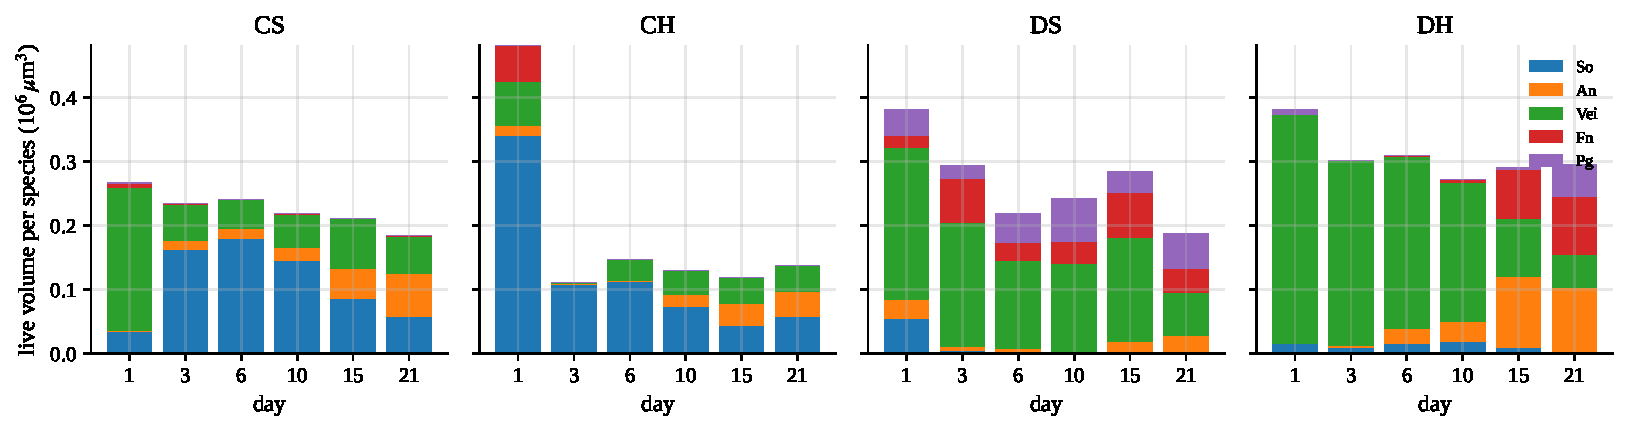
\includegraphics[width=\linewidth]{fig_vol_species.pdf}
\end{column}
\end{columns}
\vspace{4pt}
\begin{itemize}\small
  \item 左：生きた割合は群集全体の値（種ごとではない）。Day 1 の 0.7〜0.98 から、多くの条件で 0.35〜0.7 に下がる。
  \item 右：種ごとの生きた体積 = 体積 × 生きた割合 × 生きた菌の組成（qPCR）。常在は Vei と So、
        dysbiotic は後半に Fn と Pg が増える。推定には使っていない目安の値。
\end{itemize}
\end{frame}

% --------------------------------------------------------
\begin{frame}{今回の結果 1：成長の速さと時間の対応}
\begin{columns}[c]
\begin{column}{0.5\textwidth}
\centering
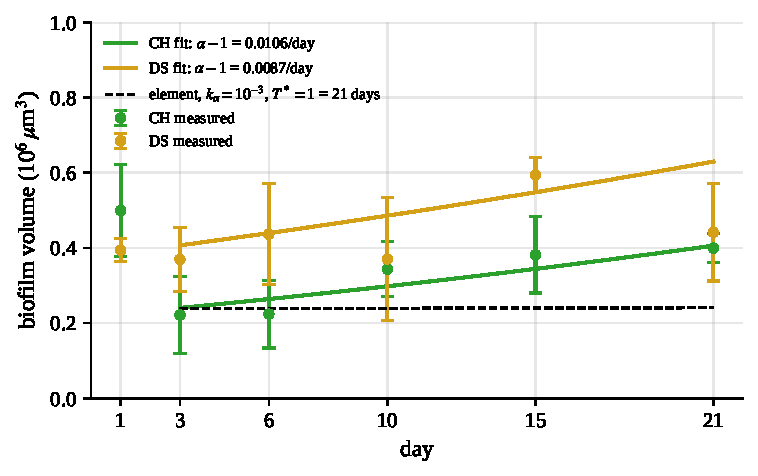
\includegraphics[width=\linewidth]{fig_vol_fit.pdf}
\end{column}
\begin{column}{0.48\textwidth}
\small
\begin{itemize}\setlength{\itemsep}{3pt}
  \item 詰まったバイオフィルム（$\phi\approx1$）では Eq.~36 から $\alpha-1=k_\alpha T^*$ と直線的に増え、
        体積は $\alpha^3$ 倍。
  \item 体積が一番小さい日（Day 3）から $V=V_0(1+r(d-d_0))^3$ を当てはめた。
  \item CH：$r=0.0106$/日（当てはまり良い）、DS：$0.0087$/日（増減あり）。
  \item 今の要素の計算（破線、$T^*=1$ = 21 日）は、ほとんど増えない。
\end{itemize}
\end{column}
\end{columns}
\pt{\textbf{成長の速さは約 0.01/日}。論文の $k_\alpha=10^{-3}$ のままなら 1 日 $\approx$ 10\,$T^*$。
修論の時間の対応（$T^*=1$ = 21 日）はそのままにして、成長の速さだけを\textbf{約 0.2/$T^*$} にするのが簡単
（$\beta$ や栄養の時間を変えずに済む）。}
\end{frame}

% --------------------------------------------------------
\begin{frame}{今回の結果 2：応力の大きさの目安}
\begin{columns}[c]
\begin{column}{0.48\textwidth}
\centering
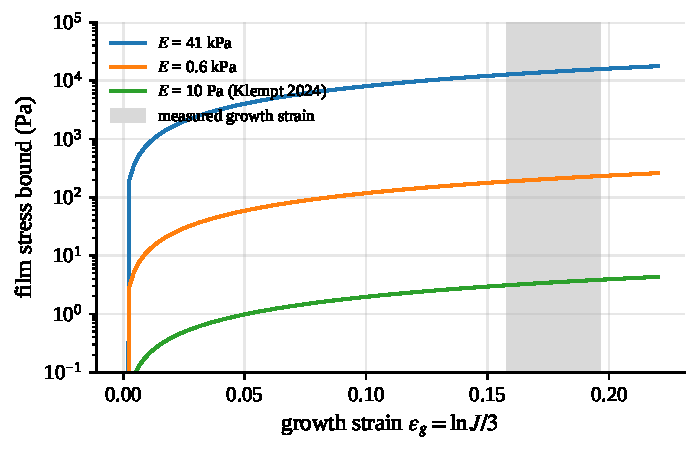
\includegraphics[width=\linewidth]{fig_vol_stress.pdf}
\end{column}
\begin{column}{0.5\textwidth}
\small
\begin{itemize}\setlength{\itemsep}{3pt}
  \item 基材に貼り付いて横に動けない薄い層：$\sigma\approx E\,\varepsilon_g/(1-\nu)$、$\nu=0.49$。
  \item 実測の成長ひずみ $\varepsilon_g=\ln J/3$ は 0.16〜0.20（灰色の帯）。
  \item $E$ = 10 Pa（論文）なら 3〜4 Pa、0.6 kPa なら 190〜230 Pa、41 kPa なら 13〜16 kPa
        （Pattem 2018 の範囲）。
  \item 今の要素の計算（シードの vM 平均 $4.7\times10^{-4}$ Pa）は、成長が小さいぶん約 1 万分の 1。
\end{itemize}
\end{column}
\end{columns}
\pt{緩和も流れもないときの\textbf{上限の目安}。FEM の結果が桁として妥当かを見る物差しになる。}
\end{frame}

% --------------------------------------------------------
\begin{frame}{注意すること}
\begin{itemize}\setlength{\itemsep}{6pt}
  \item \textbf{「300 倍の差」はモデルの誤りではない。}$T^*$ と日数の対応（修論の仮定 $s$）と $k_\alpha$ の組み合わせが、
        論文で決まっていないため。体積で、その組み合わせを決められる。
  \item \textbf{視野の体積}：1 個のコロニーの成長ではない。剥がれ、取り込み、培地交換（流れの反応器では 24 時間後）も入る。
  \item \textbf{毎回別のバイオフィルム}：同じものを追った時系列ではない。
  \item \textbf{減る部分は出せない}：CS は減り続け、CH は Day 3 まで減り、DH は Day 6 以降に減る。今の成長則
        （$\dot\alpha\ge0$）は縮まないので、剥がれや死んだ部分の分解が要る。
  \item \textbf{$\phi\approx1$ の仮定}：まばらなバイオフィルムでは、成長はもっと遅く見える。
\end{itemize}
\end{frame}

% --------------------------------------------------------
\begin{frame}{今後の使い方}
\small
\begin{tabular}{@{}p{0.03\linewidth}p{0.4\linewidth}p{0.49\linewidth}@{}}
\toprule
& 使い方 & 状況・次の一手\\
\midrule
1 & 成長則の検証：方式 (a) と (c) のどちらが体積の形に合うか & IKMHIWI03 で、体積に合わせた $\kappa$ で回す（指示書 A-5）\\
2 & 成長の速さを体積で決める（自分の仮定をデータに） & 約 0.2/$T^*$ と決めた。(c) では $\kappa\approx$ 2.3〜2.8 を回して確かめる\\
3 & 応力の大きさの物差し & 済み（上限 3 Pa〜16 kPa、$E$ による）\\
4 & 条件ごとの応力：4 条件の体積変化で成長させ、歯・インプラントで比べる & P3（慶應）の柱。DS・DH の MAP 待ち\\
5 & 生きた体積と死んだ体積を分け、生きた部分だけが成長に効くか確かめる & P3。種ごとの生きた体積を使う\\
6 & 減る部分（剥がれ・分解）をモデルに入れる & 慶應での課題。CS と DH の後半が試金石\\
\bottomrule
\end{tabular}
\vspace{6pt}
\pt{修論には、まず 1 と 2 を Outlook に一段落で（IKMHIWI03 の結果が出たら）。3 は会議の話題に。4〜6 は P3。}
\end{frame}

\end{document}
